% Adapted from UH Manoa theme by:
% UH Manoa presentation theme for beamer
% Jeff Delmerico <jeffdelmerico@gmail.com> 2012
% https://github.com/jeffdelmerico/UH_Beamer_Theme.git


\documentclass{beamer}
%\documentclass[handout]{beamer}
\usetheme{PD}

\usepackage[utf8]{inputenc}
\usepackage[absolute,overlay]{textpos}
\usepackage{helvet}
\usepackage{tikz}
\usepackage{listings,lstautogobble}
\usepackage{syntax}
\usepackage{mathrsfs}
\usetikzlibrary{tikzmark,fit,decorations.pathreplacing}

\title{Spores}
\subtitle{\newline Closures per la programmazione funzionale distribuita e type-safety}
\author{Matteo Di Pirro}
\date{17 Febbraio 2017}
\institute{Università degli Studi di Padova}

\lstset{
	autogobble=true
}

\setlength{\grammarindent}{3em}

\begin{document}

\newcommand{\turnOffNumbers}{true} %hide frame numbers in footer

\begin{frame}[noframenumbering]
\titlepage
\end{frame}

\let\turnOffNumbers\empty
\begin{frame}
	\frametitle{Outline}
	\tableofcontents
\end{frame}

\section{Introduzione}
\begin{frame}[fragile]{Distributed computing?}
	\begin{itemize}
		\item Linguaggi funzionali
	\end{itemize}
	\begin{lstlisting}[basicstyle=\fontsize{9}{9}\ttfamily]
	sendFunc :: sendPort (Int -> Int) -> Int -> ProcessM()
	sendFunc p x = sendChan p (\y -> x + y + 1)
	\end{lstlisting}
	\begin{itemize}
		\item Linguaggi Object-Oriented
		\begin{itemize}
			\item Anche il \texttt{this} deve essere serializzato
		\end{itemize}
	\end{itemize}
	\begin{figure}
		\centering
\includegraphics[scale=0.2]{distributed-computing}
	\end{figure}
\end{frame}

\section{Spore}
\begin{frame}[fragile]{Spore}
	\begin{itemize}
		\item Astrazioni che permettono di controllare l'ambiente \textit{catturato} da una closure
	\end{itemize}
	\begin{tikzpicture}[remember picture,overlay]
	\draw<2-> [decorate,decoration={brace,amplitude=10pt,raise=4pt},yshift=0pt]
	(5.5,-0.85) -- (5.5,-2.2) node [white,midway,xshift=1.5cm] {\footnotesize{Header}};
	\draw<3-> [decorate,decoration={brace,amplitude=10pt,raise=4pt},yshift=0pt]
	(5.5,-2.2) -- (5.5,-3.65) node [white,midway,xshift=1.5cm] {\footnotesize{Body}};
	\end{tikzpicture}
	\begin{lstlisting}
		spore {
		    val y1: S1 = <expr1>
		    ...
		    val yn: Sn = <exprn>
		    (x: T) => {
		        // corpo
		    }
		}
	\end{lstlisting}
\end{frame}	
\begin{frame}{Sintassi}
	\begin{grammar}
		<t> ::= \texttt{spore} $\{\overline{x: T = t}$; $\overline{pn}$; (x: T) $\rightarrow$ t$\}$
		\alt \texttt{import} $pn$ \texttt{in} $t$
		\alt $t$ \texttt{compose} $t$
	\end{grammar}	
	
	\begin{onlyenv}<2->
		\begin{grammar}
			<v> ::= \texttt{spore} $\{\overline{x: T = v}$; $\overline{pn}$; (x: T) $\rightarrow$ t$\}$
		\end{grammar}
	\end{onlyenv}
	
	\begin{onlyenv}<3->
		\begin{grammar}
			<T> ::= $\mathcal{S}$
			
			<$\mathcal{S}$> ::= T $\rightarrow$ T \{\texttt{type} $\mathcal{C}$ = $\overline{T}$; $\overline{pn}$\}
			\alt T $\rightarrow$ T \{\texttt{type} $\mathcal{C}$; $\overline{pn}$\}
		\end{grammar}
	\end{onlyenv}
	
	\only<4->{
		$\mathcal{P} \in pn \rightarrow \mathcal{T}$ \\
		$\mathcal{T} \in \mathcal{P}(T)$
	}
	
	\begin{onlyenv}<5->
		\begin{grammar}
			<$\Gamma$> ::= $\overline{x: T}$
			
			<$\Delta$> ::= $\overline{pn}$
		\end{grammar}
	\end{onlyenv}
\end{frame}
\begin{frame}{Proprietà}
	\begin{itemize}
		\item Impongono vincoli aggiuntivi 
		\item Limitano (a compile-time):
		\begin{itemize}
			\item I tipi ''catturabili'' dall'oggetto Spore
			\item Il tipo di un parametro Spore
		\end{itemize}
		\item \texttt{import}
		\item ''Componibili'' a piacere 
	\end{itemize}
	\only<2->{
		\vspace{0.5cm}
		\centering Se $T <: T'$ e $T' \in P(pn)$ allora $T \in P(pn)$
	}
\end{frame}

\section{Typing}
\begin{frame}{Regole di Typing}
	\begin{figure}
		\centering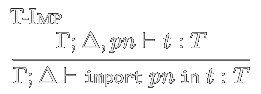
\includegraphics[scale=0.5]{timp}
	\end{figure}
	
	\begin{onlyenv}<2->
		\begin{figure}
			\centering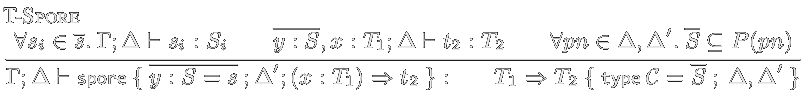
\includegraphics[scale=0.4]{tspore}
		\end{figure}
	\end{onlyenv}
	
	\begin{onlyenv}<3->
		\begin{figure}
			\centering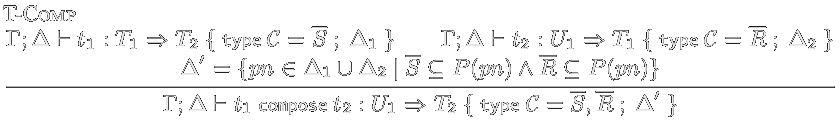
\includegraphics[scale=0.35]{tcomp}
		\end{figure}
	\end{onlyenv}
\end{frame}
\begin{frame}{Regole di Subtyping}
	\begin{figure}
		\centering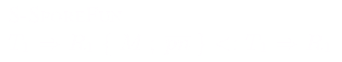
\includegraphics[scale=0.5]{ssporefun}
	\end{figure}
	
	\begin{onlyenv}<2->
		\begin{figure}
			\centering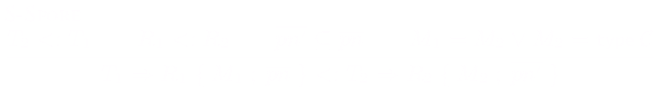
\includegraphics[scale=0.45]{sspore}
		\end{figure}
	\end{onlyenv}
\end{frame}

\section{Semantica operazionale}

\section{Soundness}

\section{Tipi esclusi}

\appendix
\makethanks
\renewcommand{\turnOffNumbers}{true} %hide frame numbers in footer
% extra slides
\end{document}
